\section{Exercise 3: AM Communications via USRP}
\label{sec:ex3}

\subsection*{Task 1: Functional Understanding of Tx and Rx Modules}
The first task is to explain how the provided USRP transmitter and receiver modules operate from their block diagrams.

\subsection*{USRP Transmitter (TX) Module}
Figure~\ref{fig:usrp_tx_vi} shows the TX VI.
\begin{figure}[H]
\centering
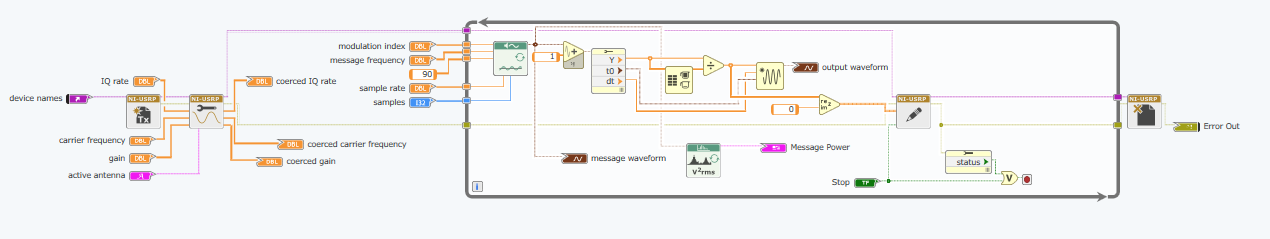
\includegraphics[width=\linewidth]{figures/usrp_tx_vi.png}
\caption{USRP AM transmitter VI block diagram.}
\label{fig:usrp_tx_vi}
\end{figure}

Functionally, the TX VI performs the following steps:
\begin{enumerate}
\item Opens a TX session to the selected device.
\item Configures radio parameters (IQ rate, carrier frequency, gain, active antenna), and reports coerced values.
\item Inside a while loop, generates the message waveform from the set message frequency, sample rate, and sample count.
\item Applies the modulation index to form the AM baseband signal and prepares complex IQ samples (real path carrying the AM waveform).
\item Streams data continuously using \texttt{niUSRP Write Tx Data}, so the USRP upconverts and transmits at the configured RF carrier.
\item Stops cleanly and closes the session when the stop control is pressed.
\end{enumerate}

\subsection*{USRP Receiver (RX) Module}
Figure~\ref{fig:usrp_rx_vi} shows the RX VI.
\begin{figure}[H]
\centering
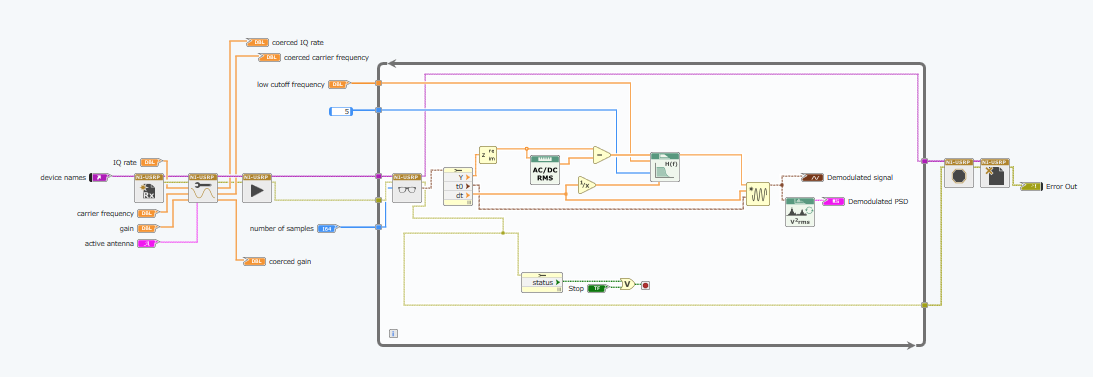
\includegraphics[width=\linewidth]{figures/usrp_rx_vi.png}
\caption{USRP AM receiver VI block diagram.}
\label{fig:usrp_rx_vi}
\end{figure}

Functionally, the RX VI performs:
\begin{enumerate}
\item Opens an RX session and configures IQ rate, carrier frequency, gain, and active antenna.
\item Initiates reception and enters a while loop to fetch blocks of received samples.
\item Uses \texttt{niUSRP Fetch Rx Data} to get baseband data from the USRP.
\item Applies baseband post-processing in the VI: low-pass filtering, DC removal, and amplitude handling, then computes PSD.
\item Displays demodulated signal (time domain) and demodulated PSD (frequency domain).
\item Aborts acquisition and closes the session cleanly on stop.
\end{enumerate}

\subsection*{How TX and RX Work Together}
The TX module provides the USRP with baseband IQ data that represent the AM signal; the USRP hardware performs RF transmission.  
At the receiver, the USRP returns baseband data centered on the configured carrier, and the RX VI finalizes message recovery with filtering/offset removal and visualization.  
This is why the modules are mainly configuration, streaming, and baseband-processing pipelines rather than full RF implementations in LabVIEW code.

\subsection*{Task 2: Single-Tone Transmission and Recovery}
For Task 2, the transmitter is configured to send a single-tone AM message and the receiver output is observed in both time and frequency domains.

\begin{figure}[H]
\centering
\begin{subfigure}{0.49\linewidth}
\centering
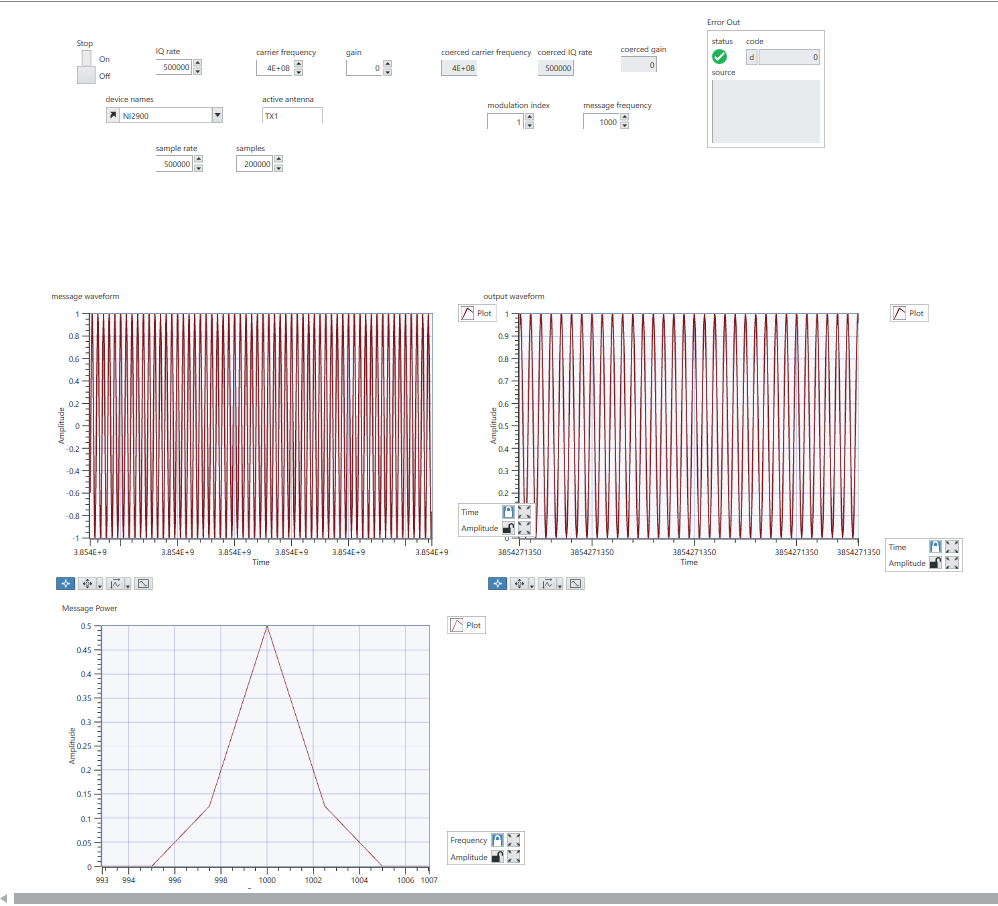
\includegraphics[width=\linewidth]{figures/ex3_task2_tx_panel.png}
\caption{USRP TX panel during single-tone transmission.}
\label{fig:ex3_task2_tx}
\end{subfigure}
\hfill
\begin{subfigure}{0.49\linewidth}
\centering
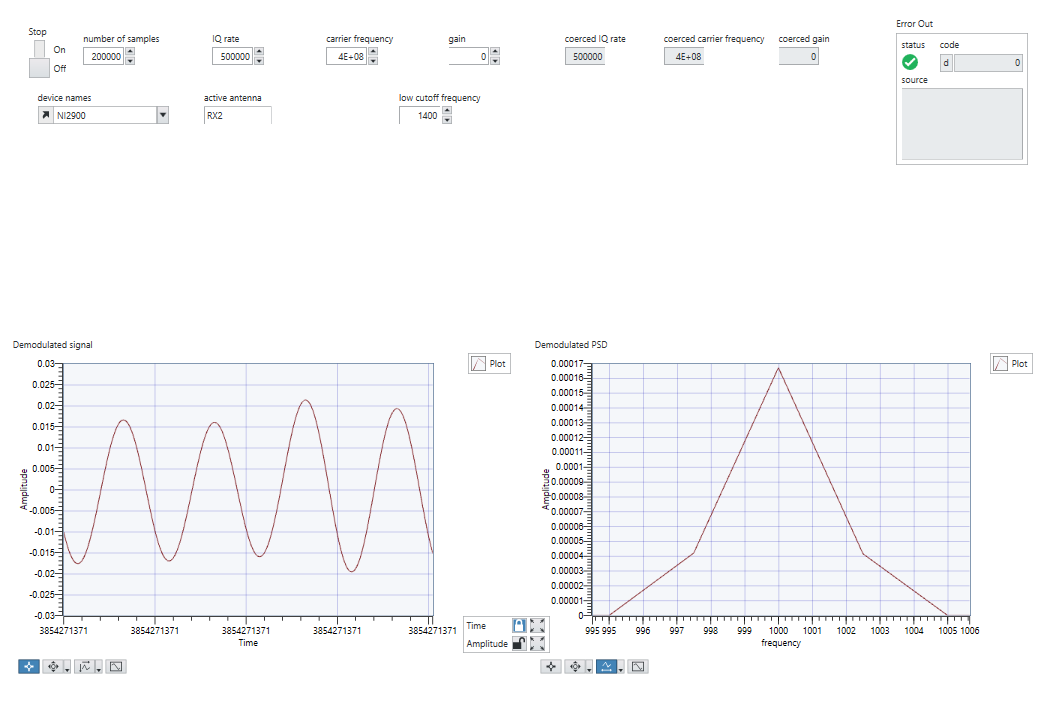
\includegraphics[width=\linewidth]{figures/ex3_task2_rx_panel.png}
\caption{USRP RX panel showing demodulated signal and PSD.}
\label{fig:ex3_task2_rx}
\end{subfigure}
\caption{Exercise 3 Task 2 capture (transmission and reception).}
\label{fig:ex3_task2}
\end{figure}

\textbf{Observed result:}
\begin{itemize}
\item The demodulated time-domain waveform is sinusoidal, confirming successful AM message recovery.
\item The demodulated PSD shows a dominant single peak at the message frequency (in the provided capture, near \(1~\text{kHz}\)).
\end{itemize}

This confirms that the TX/RX chain is operating correctly: the transmitter sends an AM-modulated tone and the receiver recovers the baseband message.

\subsection*{Task 3: Noise Effect Versus Modulation Index}
To study noise sensitivity, receiver gain was increased and the modulation index was varied. The captured results for \(\mu=1\), \(\mu=0.5\), and \(\mu=0.2\) are shown in Figure~\ref{fig:ex3_task3}.

\begin{figure}[H]
\centering
\begin{subfigure}{0.49\linewidth}
\centering
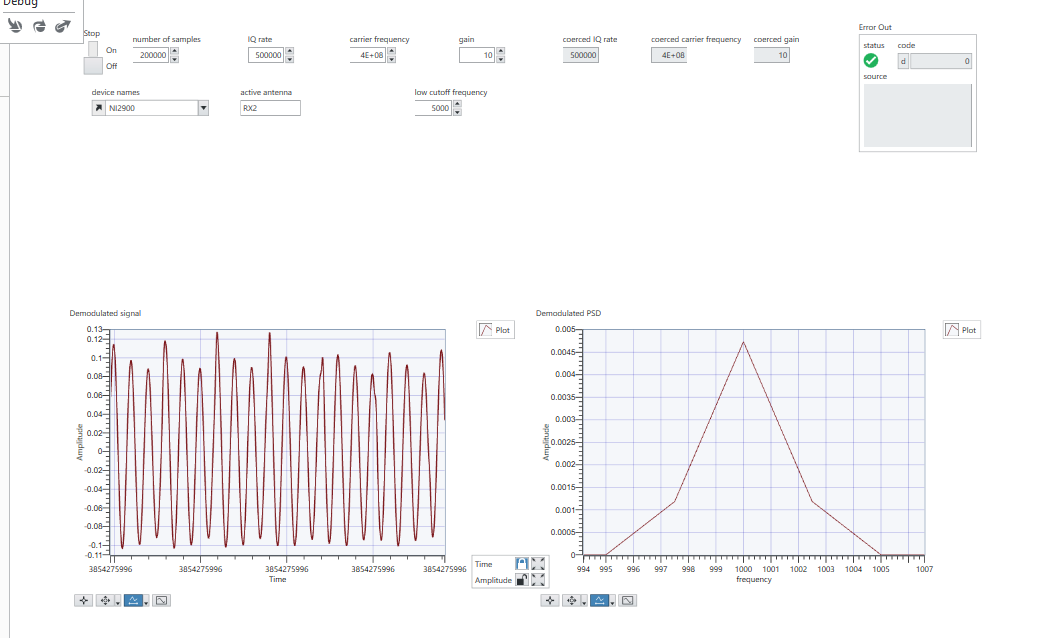
\includegraphics[width=\linewidth]{figures/ex3_task3_mu_1.png}
\caption{\(\mu=1\)}
\label{fig:ex3_mu1}
\end{subfigure}
\hfill
\begin{subfigure}{0.49\linewidth}
\centering
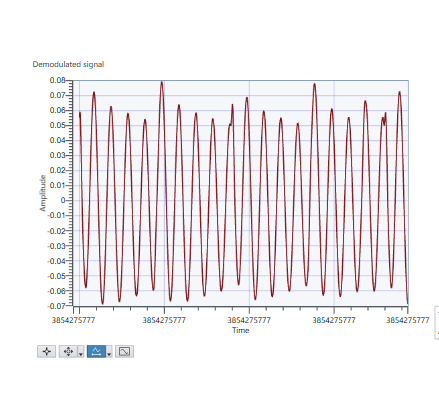
\includegraphics[width=\linewidth]{figures/ex3_task3_mu_05.png}
\caption{\(\mu=0.5\)}
\label{fig:ex3_mu05}
\end{subfigure}

\vspace{0.5em}

\begin{subfigure}{0.65\linewidth}
\centering
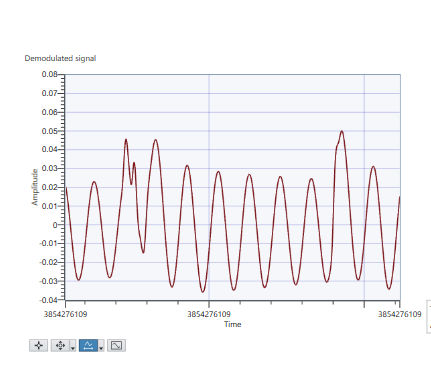
\includegraphics[width=\linewidth]{figures/ex3_task3_mu_02.png}
\caption{\(\mu=0.2\)}
\label{fig:ex3_mu02}
\end{subfigure}
\caption{Exercise 3 Task 3: demodulated signal under increased receiver gain for different modulation indices.}
\label{fig:ex3_task3}
\end{figure}

\textbf{What changes as \(\mu\) decreases?}
\begin{itemize}
\item At \(\mu=1\), the recovered sinusoid is strongest relative to noise and appears the cleanest.
\item At \(\mu=0.5\), the desired signal amplitude is lower, so fluctuations/noise become more visible.
\item At \(\mu=0.2\), the message is weakest and noise is clearly noticeable, with visible irregular perturbations in the waveform.
\end{itemize}

\textbf{Why this happens:} the demodulated message component scales with modulation index, so reducing \(\mu\) reduces recovered signal amplitude while receiver noise/interference does not reduce proportionally. Therefore, output SNR decreases as \(\mu\) decreases.

\textbf{Conclusion for Task 3:} in these results, noise becomes clearly noticeable from approximately \(\mu \approx 0.2\) (and starts to become apparent already near \(\mu=0.5\)).
